\newpage

\section{Methodology}

\subsection{Conceptual Design}

\subsubsection{Robot Chassis}
In mobile robots, there is a wide of range of chassis mechanism and differential types of wheels including mecanum wheels, omni and caster wheels.
The chassis is assembled using 20$\times$20 mm T-slot aluminum frame due to its strength-weight-ratio and modularity. The wheels are 150 mm in diameter
and pneumatic.

\begin{figure}[H]
    \centering
    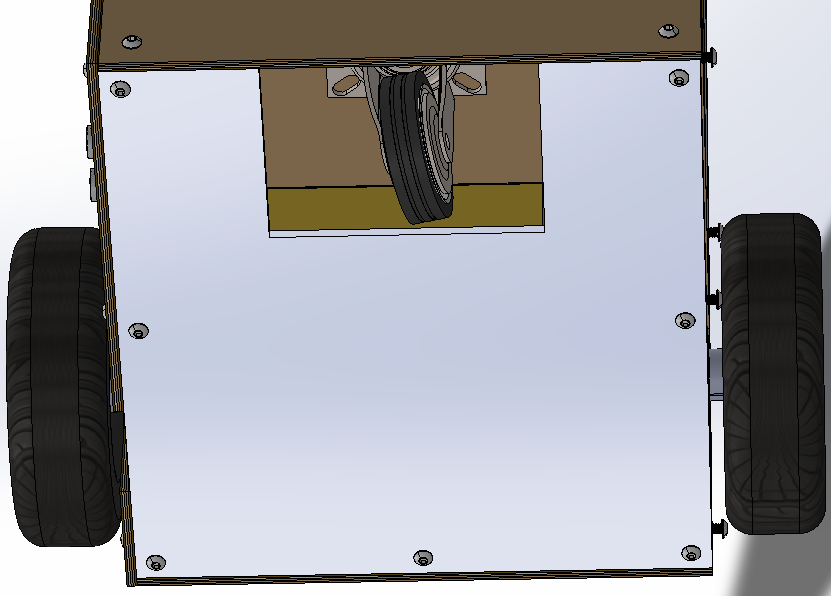
\includegraphics[width=5.5in]{pics/diff.png} 
    \caption{Differential drive chassis}\label{diff_cart}
\end{figure}

\noindent The robot has multiple compartments for medicine storage and delivery purposes. The height of the robot is 450mm, but will be reduced to
optimize costs. There are two layers: the lower layer houses the low-level actuators including motor drivers, motors, and battery,
while the upper layer contains the Single Board Computer (SBC) and Microcontroller Unit (MCU). A LiDAR sensor is mounted on the topmost 
section of the robot. The robot is enclosed with plywood panels attached to the 20$\times$20mm aluminum frame profiles. Emergency
stop buttons are positioned on the rear of the robot, and a switch will be mounted on the front panel to confirm delivery.

\begin{figure}[H]
    \centering
    \begin{minipage}{0.45\textwidth}
        \centering
        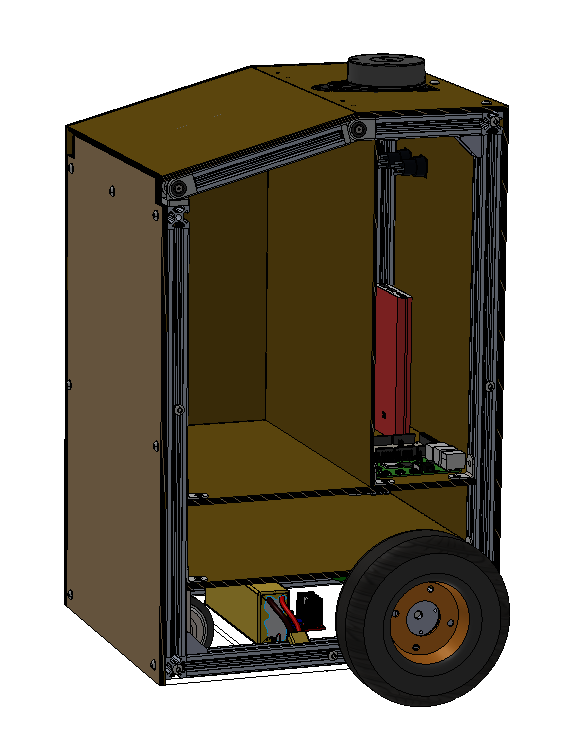
\includegraphics[width=2.9in]{pics/front_cart.png}
    \end{minipage}\hfill
    \begin{minipage}{0.45\textwidth}
        \centering
        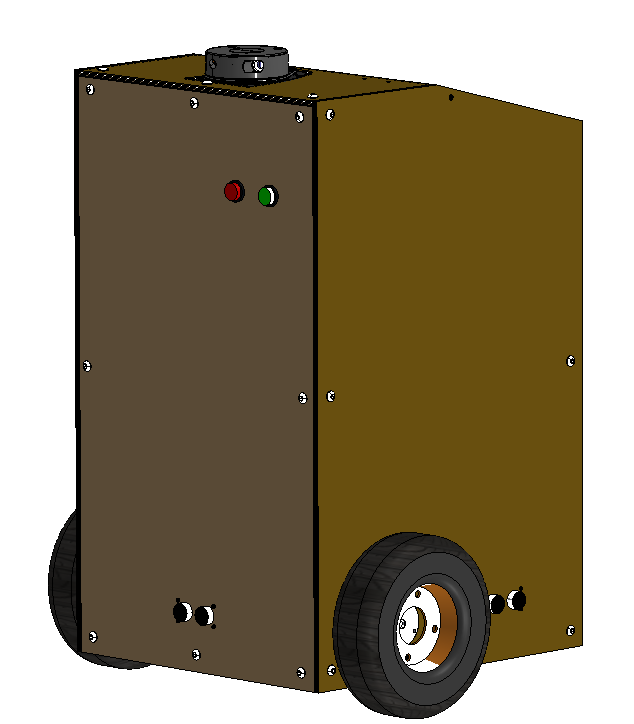
\includegraphics[width=2.9in]{pics/back_cart.png}
    \end{minipage}\hfill
    \caption{Isometric views of the robot}\label{back_cart}
\end{figure}

\vspace{-1.2em}

\subsubsection{Kinematic Model}
For this project, there are two independent driving wheels which are equipped with either one or two passive wheel(s) of caster type. The wheels
can turn at different speeds and they are attached to the robot on the same axis hence they can govern the direction of movement of the robot
as well as its speed. The wheels have radius $r$, separated by a wheelbase of length $L = 2b$, where $b$ is half the distance between the wheels. The robot's motion is controlled by varying the angular velocities of the left and right wheels, denoted by $\dot{\theta}_l$ and $\dot{\theta}_r$, respectively.

\begin{figure}[H]
    \begin{minipage}{0.55\textwidth}
        \begin{enumerate}[label=\alph*)]
            \item Equal speed in both wheels = forward motion
            \item Equal speed in both wheels = backward motion
            \item Equal speed in both wheels, but in opposite\\ directions
            \item Higher speed for left wheel = robot turns right
            \item Higher speed for right wheel = robot turns left
        \end{enumerate}
    \end{minipage}
    \hfill
    \begin{minipage}{0.45\textwidth}
        \centering
        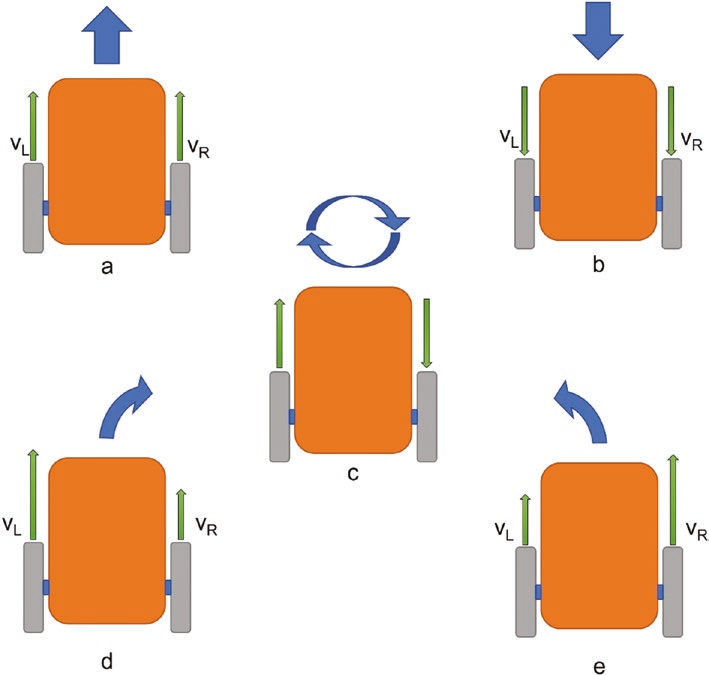
\includegraphics[width=1.7in]{pics/kine.png}
        \caption[Motion description of a two-wheel differential drive chassis]{Visual description~\cite{subramanian2023autonomous}}
        \label{kine1}
    \end{minipage}
\end{figure}

\vspace{-1em}

\noindent Two coordinate frames are defined to describe the robot's motion:

\vspace{-0.8em}

\begin{enumerate} 
    \setlength\itemsep{-0.5em}
    \item \textbf{Inertial Frame} $(X, Y)$: A global, fixed reference frame. 
    \item \textbf{Body Frame} $(x, y)$: A frame attached to the robot, with the $x$-axis pointing forward and the $y$-axis pointing to the left. 
\end{enumerate}


\begin{figure}[H]
    \centering
    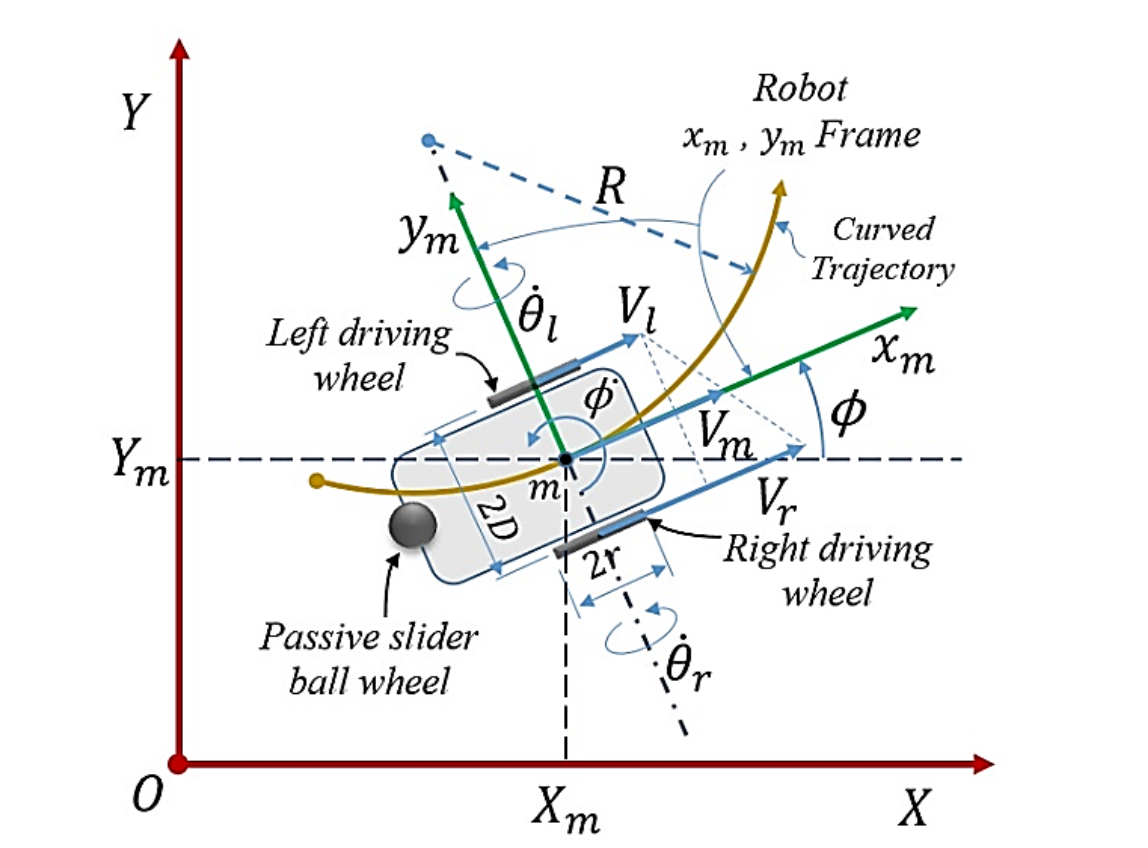
\includegraphics[width=4.0in]{pics/x_y.png}
    \caption[Kinematic structure of a differential drive]{Kinematic structure of a differential drive~\cite{azevedo2018lidar}}
\end{figure} 


\noindent The robot's pose in the inertial frame is represented by the vector $\mathbf{p} = [X_m, Y_m, \phi]^\top$, where $X_m$ and
$Y_m$ are the position coordinates, and $\phi$ is the orientation angle between the robot's heading and the inertial $X$-axis. Assumptions are taken into consideration that the robot wheels are rolling without slipping and the centre of mass of the robot is
located at the axis of the wheels rotation. Under the no-slfip assumption (i.e., the wheels roll without lateral slipping), the
robot's instantaneous motion in its body frame can be described by:

\vspace{-0.25em}

\begin{equation} \begin{aligned} \dot{x} &= v, \ \dot{y} &= 0, \ \dot{\phi} &= \omega, \end{aligned} \end{equation}

where:

\begin{itemize}
    \setlength\itemsep{-0.5em}
    \item $v$ is the linear velocity along the robot's forward direction ($x$-axis),
    \item $\omega$ is the angular velocity around the vertical axis (rotation rate),
    \item $\dot{x}$ and $\dot{y}$ are the velocities along the $x$ and $y$ axes of the body frame,
    \item $\dot{\phi}$ is the rate of change of the robot's orientation,
    \item \( r \) be the radius of each wheel,
    \item \( L = 2b \) be the wheelbase (the distance between the two wheels),
    \item \( \dot{\theta}_l \) and \( \dot{\theta}_r \) be the angular velocities of the left and right wheels, respectively.
\end{itemize}


\noindent For motion analysis, the robot’s linear velocity \( v \) and angular velocity \( \omega \) about its center are given by:

\begin{equation}
v = \frac{r}{2} \left( \dot{\theta}_r + \dot{\theta}_l \right)
\label{eq:linear_velocity}
\end{equation}

\vspace{-0.25em}

\begin{equation}
\omega = \frac{r}{L} \left( \dot{\theta}_r - \dot{\theta}_l \right)
\label{eq:angular_velocity}
\end{equation}


\noindent For velocity analysis, the condition $\dot{y} = 0$ arises because, in the body frame, the robot cannot move sideways without wheel slippage. The wheels can only induce motion along the forward direction and rotation about the robot's center.
The velocities \( \dot{X} \), \( \dot{Y} \), and \( \dot{\phi} \) in the inertial frame are related to the body frame velocities \( v \) and \( \omega \) by:

\begin{equation}
\begin{bmatrix} \dot{X} \\ \dot{Y} \\ \dot{\phi} \end{bmatrix}
=
\begin{bmatrix} \cos \phi & 0 \\ \sin \phi & 0 \\ 0 & 1 \end{bmatrix}
\begin{bmatrix} v \\ \omega \end{bmatrix}
\label{eq:transformation}
\end{equation}


\noindent Transfomring the velocities from the body frame to the inertial frame gives

\begin{equation}
    \begin{bmatrix} \dot{X} \\ \dot{Y} \\ \dot{\phi} \end{bmatrix}
    =
    \begin{bmatrix} v\cos \\v\sin \\ \omega \end{bmatrix}
    \label{eq:transformation2}
\end{equation}
    



\noindent Using wheel encoders, the angular velocities \( \dot{\theta}_l \) and \( \dot{\theta}_r \) can be approximated as:

\begin{equation}
\dot{\theta}_l = \frac{\Delta \theta_l}{\Delta t}, \quad \dot{\theta}_r = \frac{\Delta \theta_r}{\Delta t}
\label{eq:encoder_velocities}
\end{equation}

\noindent where \( \Delta \theta_l \) and \( \Delta \theta_r \) are the incremental angular
displacements of the left and right wheels over the sampling interval \( \Delta t \).Substituting
Equation~\eqref{eq:encoder_velocities} into Equations~\eqref{eq:linear_velocity} 
and \eqref{eq:angular_velocity} yields the following:

\begin{equation}
v = \frac{r}{2 \Delta t} \left( \Delta \theta_r + \Delta \theta_l \right)
\label{eq:linear_velocity_encoder}
\end{equation}

\begin{equation}
\omega = \frac{r}{L \Delta t} \left( \Delta \theta_r - \Delta \theta_l \right)
\label{eq:angular_velocity_encoder}
\end{equation}

\noindent These equations allow computation of the robot's linear and angular velocities based on encoder data.


\newpage
\subsection{Hardware Implementation}



\subsubsection{Sensors design specifications}
For this section, the sensors to be used in the robot are analysed and their specifications are presented while determining the proper placement of each of the sensor element on the robot. 
As sensors' workings, their algorithms and how they interact, this will be further discussed in the software implementation section. 
To achieve navigation, one of the most popular sensors used is the LiDAR. 



\begin{table}[h]
    \begin{minipage}{0.5\textwidth}
    \centering
    \renewcommand{\arraystretch}{2.0}
    \setlength{\tabcolsep}{4.4pt}
    \footnotesize
    \begin{tabular}{|p{3cm}|p{4.4cm}|}
      \hline
      \rowcolor[gray]{0.8} 
      \textbf{Parameter} & \textbf{Value} \\
      \hline
      Measuring Range & 0.15m - 12m \\
      \hline
      Rotational Speed & 5.5Hz \\
      \hline
      Scanning Angle & 360$^{\circ}$ \\
      \hline
      Scanning Frequency & 10Hz \\
      \hline
      System Voltage & 5V \\
      \hline
      System Current & 100mA \\
      \hline
      Dimensions & 96.8mm x 70.3mm x 55mm \\
      \hline
      Sampling frequency & 8K \\      
      \hline
      Angular Resolution & $\leq 1^{\circ}$ \\
      \hline
      Output & UART Serial (3.3V) \\
      \hline
      Temperature Range & 0$^{\circ}$C - 40$^{\circ}$C \\
      \hline
      Range Resolution & $\leq 1\%$ of the range ($\leq 12m$), $\leq 2\%$ of the range (12m - 16m) \\
      \hline
    \end{tabular}
    \end{minipage}
    \begin{minipage}{0.55\textwidth}
        \centering
        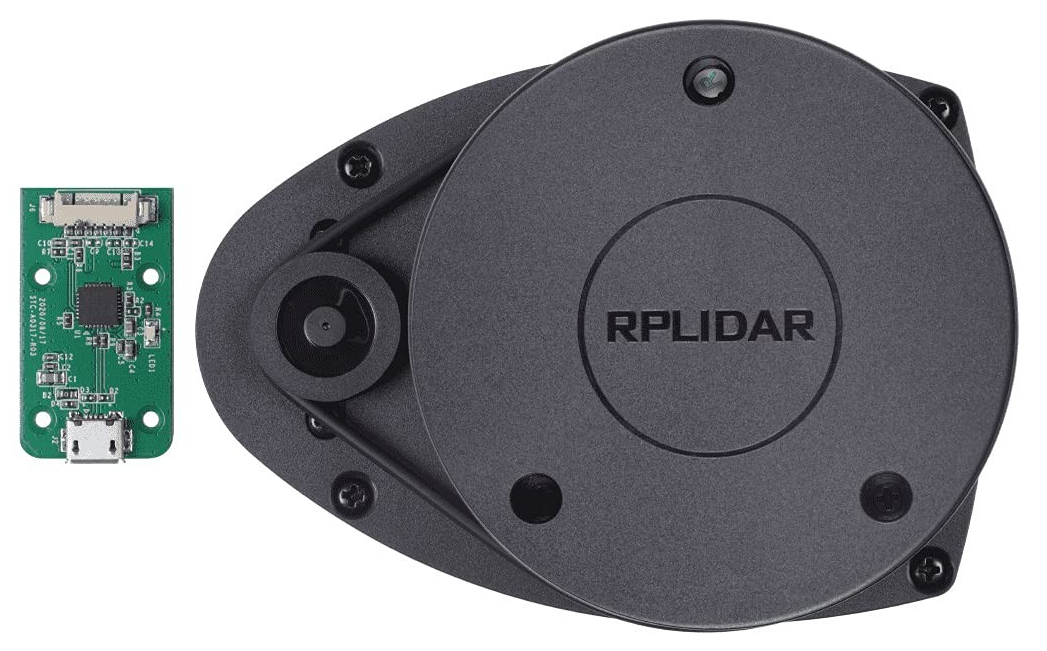
\includegraphics[width=\linewidth, angle=90]{pics/lidar.png}
    \end{minipage}\hfill
    \caption{RPLiDAR A1 M8 and its basic operating parameters}\label{tab:lidar}
\end{table}



\noindent RP LiDAR A1 M8 as shown in \figref{tab:lidar} is a 2D LiDAR sensor that performs 360-degree scanning with a range of 12 meters.
The sensor will be connected to the Raspberry Pi 4 via USB and powered by a 5V supply from the buck converter. LiDARs typically have a vertical measurement range~\cite{azevedo2018lidar}, thus requires it
placed at a certain height to avoid obstacles from the robot's side covers or the ground. To ensure this is achieved the LiDAR will be mounted on a 3D printed bracket that is attached on top of the robot at a 
450mm height.

\vspace{1.0em}
\begin{figure}[H]
    \centering
    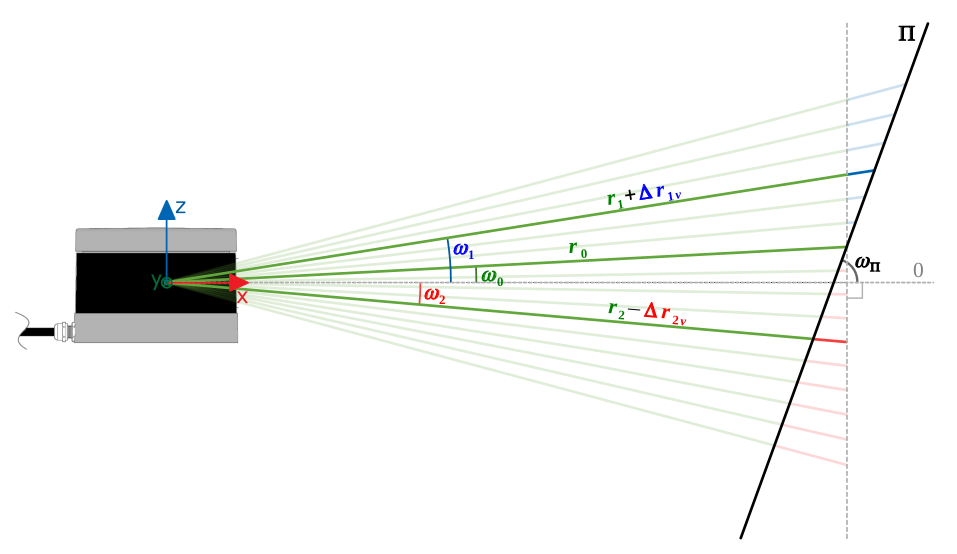
\includegraphics[width=3.8in]{pics/vertical.png}
    \caption[Vertical measurement of a LiDAR]{Vertical measurements of a LiDAR~\cite{azevedo2018lidar}}\label{vert}
\end{figure} 


\noindent For more safety on the autonomous navigation, it should also be accessible from obstacles throughout the horizontal plane to maximize its field of view. 
Thus incorporating ultrasonic sensors, Time of Flight sensor and IMU is essential so as to achieve fault-tolerant redundancy that helps other sensors~\cite{CANADASARANEGA2024100606}.
Ultrasonic sensors used high-frequency sound waves to detect objects around the the robot's perimeter. HC-SR04 is a popular ultrasonic sensor that has a range of 2cm to 400cm.
VL53L0X is a Time of Flight sensor that uses a laser to measure the distance between the robot and an object. It has a range of up to 2 meters. This sensor will be placed 
in front of the robot bumper while the three ultrasonics will be mounted on sides and the robot's rear. The Inertial Measurement Unit (IMU) integrates three types of sensors into a single
device: accelerometer, gyroscope, and a magnetometer. MPU-9250 is a popular IMU chosen for this project. It is 9-DOF meaning the sensor can measure in three-axis; acceleration (x,y,z), angular velocity (roll, pitch, yaw), and magnetic field(x,y,z).
The main reason why the IMU is used is to provide the robot with orientation and position data, that maintain accuracy of localization on robot thus making it much smoother.


\vspace{1.0em}

\begin{figure}[H]
    \centering
    \begin{minipage}{0.3\textwidth}
        \centering
        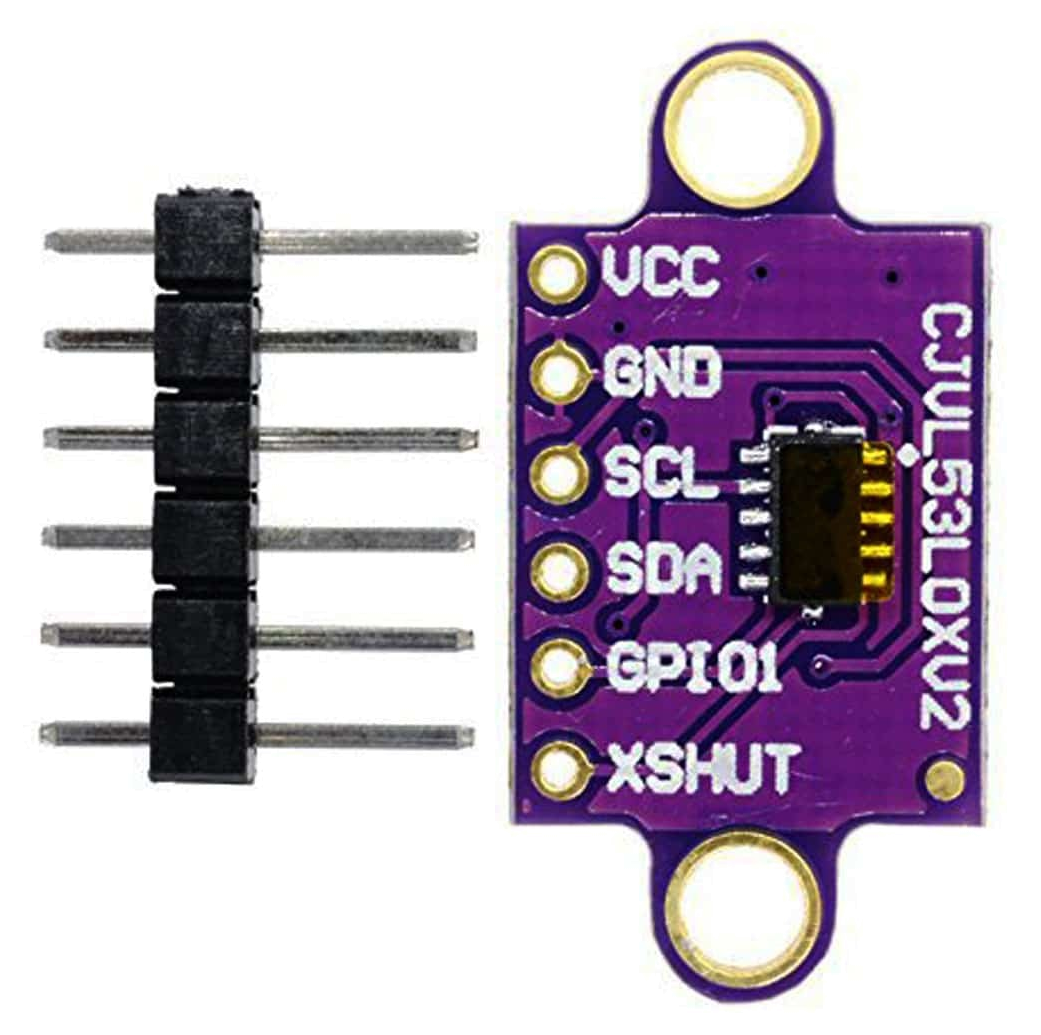
\includegraphics[width=\linewidth]{pics/tof.png}
        \caption{Time of Flight}\label{tof}
    \end{minipage}\hfill
    \begin{minipage}{0.3\textwidth}
        \centering
        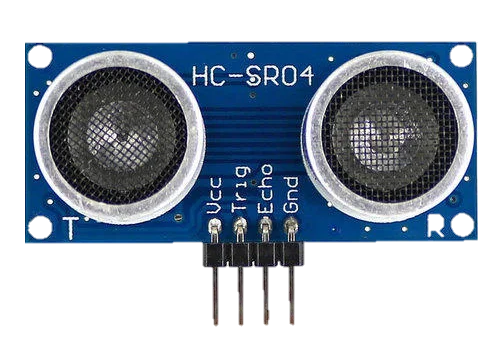
\includegraphics[width=\linewidth]{pics/hcrs04.png}
        \caption{HCR-S04}\label{ultra}
    \end{minipage}\hfill
    \begin{minipage}{0.3\textwidth}
        \centering
        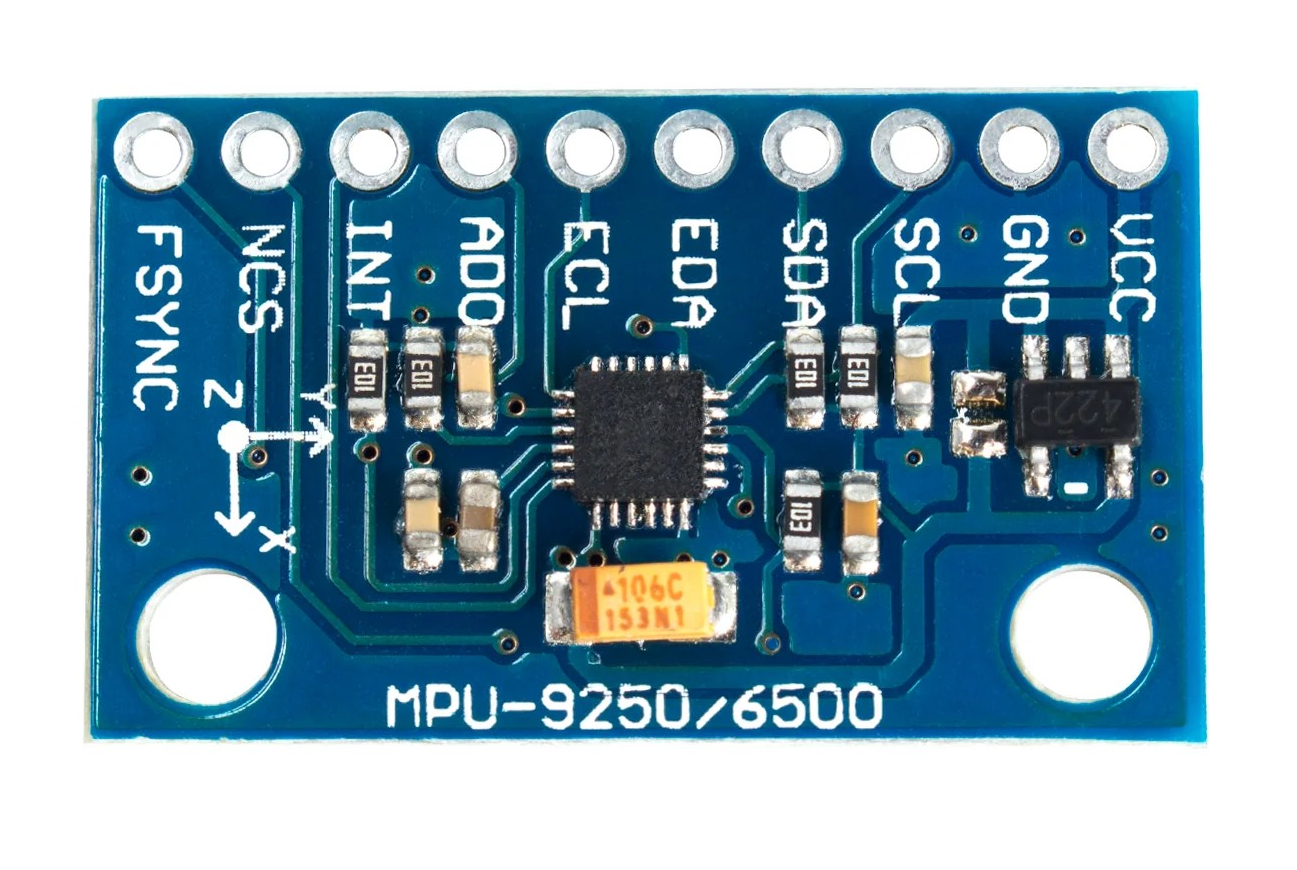
\includegraphics[width=\linewidth]{pics/mpu.png}
        \caption{MPU-9250 IMU}\label{mpu}
    \end{minipage}
    \caption{Proximity sensors used in the project}\label{prox}
    \label{fig:lidar_side_by_side}
\end{figure}

\newpage


\subsubsection{Onboard Computer}

\vspace{-0.8em}

A Raspberry Pi 4 is chosen as the onboard computer for this project, working alongside an ESP32 microcontroller. While the Raspberry Pi handles high-level processing and navigation tasks, the ESP32 is responsible for low-level control functions including motor control and sensor interfacing.

\begin{table}[h]
    \begin{minipage}{0.6\textwidth}
        \centering
        \renewcommand{\arraystretch}{2.0}
        \setlength{\tabcolsep}{4.4pt}
        \footnotesize
        \begin{tabular}{|p{2.9cm}|p{6.4cm}|}
          \hline
          \rowcolor[gray]{0.8} 
          \textbf{Parameter} & \textbf{Value} \\
          \hline
          SoC & Broadcom BCM2711, Cortex-A72 (ARM v8) 64-bit SoC @ 1.8GHz \\
          \hline
          Memory & 8GB LPDDR4-3200 SDRAM (micro SD card slot) \\
          \hline
          Wireless & 2.4 GHz and 5.0 GHz IEEE 802.11ac wireless, Bluetooth 5.0, BLE \\
          \hline
          Audio/Video & 4-pole stereo audio and composite video port \\
          \hline
          Video & H.265 (4kp60 decode) \newline H264 (1080p60 decode, 1080p30 encode) \\
          \hline
          Power Supply & 5VDC, 3A, Power over Ethernet (PoE) \\
          \hline
          Temperature Range & 0 – 50 $^\circ$C ambient \\
          \hline
        \end{tabular}
    \end{minipage}
    \begin{minipage}{0.47\textwidth}
        \centering
        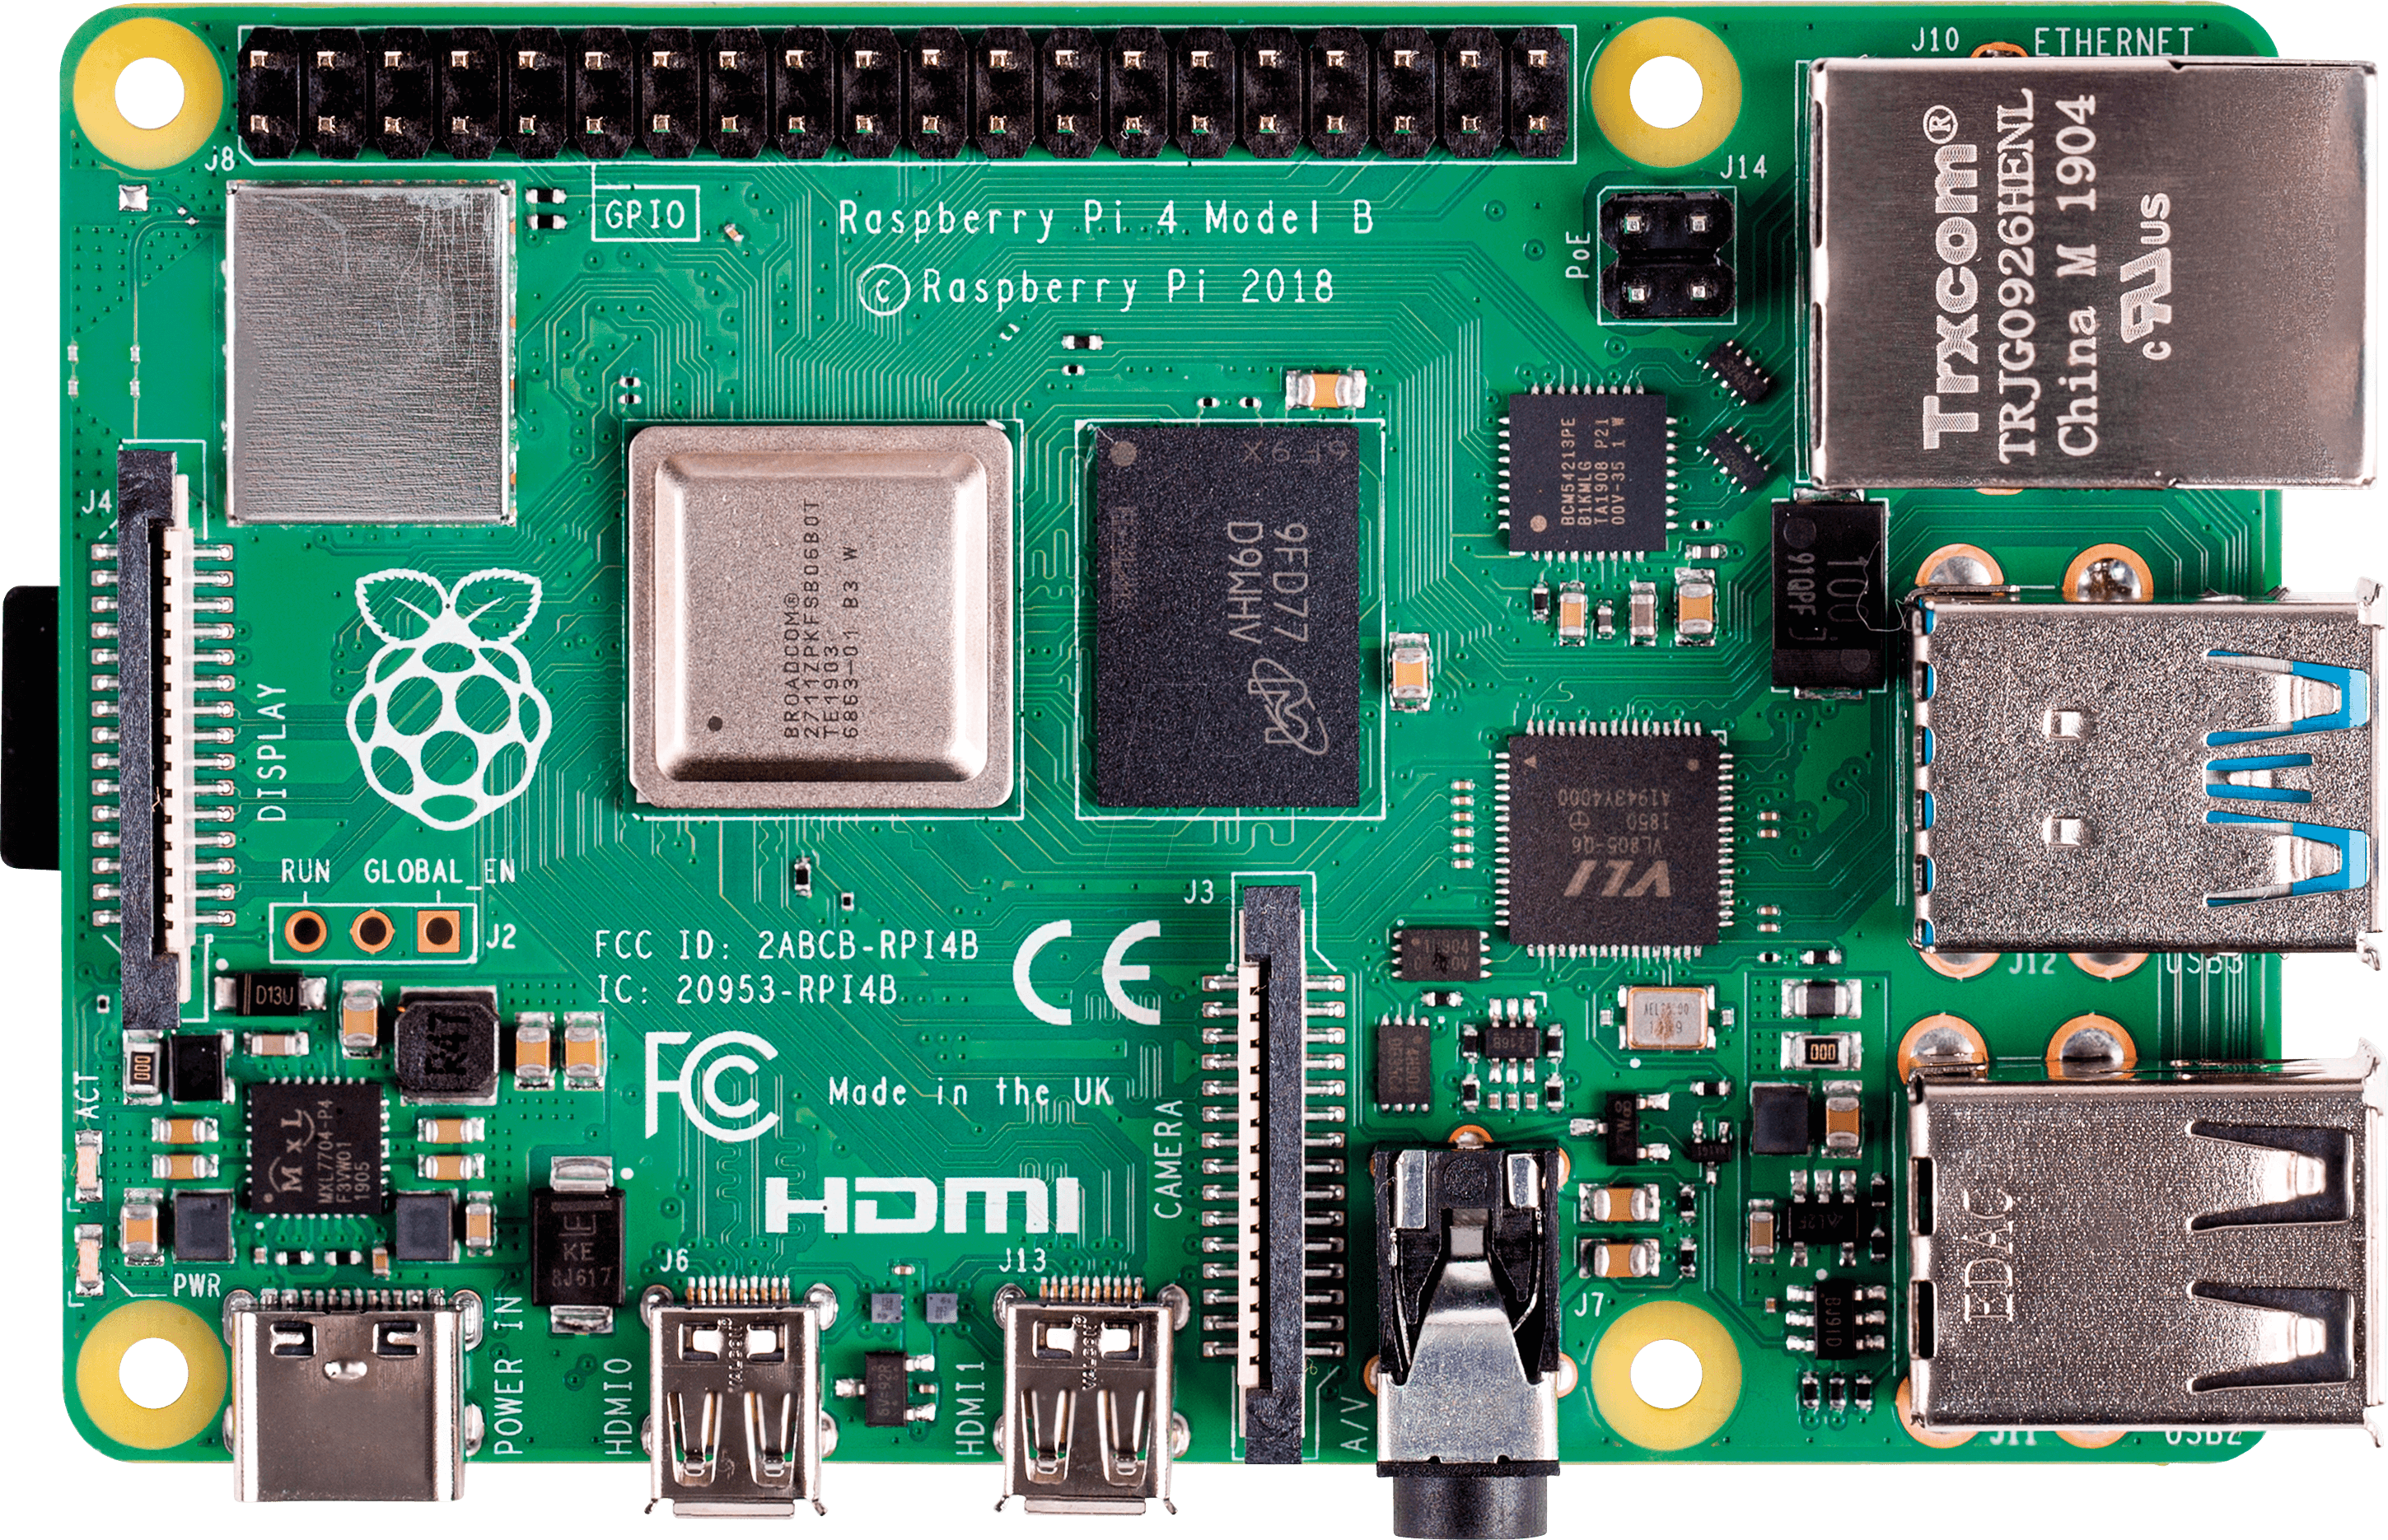
\includegraphics[width=\linewidth, angle=270]{pics/RPI4B.png}
    \end{minipage}\hfill
    \caption{Raspberry Pi 4 Model B and its specifications}\label{tab:rpi4_specs}
\end{table}



\vspace{2em}

\begin{table}[h]
    \begin{minipage}{0.6\textwidth}
        \centering
        \renewcommand{\arraystretch}{2.0}
        \setlength{\tabcolsep}{4.4pt}
        \footnotesize
        \begin{tabular}{|p{2.9cm}|p{6.4cm}|}
          \hline
          \rowcolor[gray]{0.8} 
          \textbf{Parameter} & \textbf{Value} \\
          \hline
          SoC & ESP-WROOM-32 module \\
          \hline
          Processor & Dual-core 32-bit processor with built-in 2.4 GHz Wi-Fi and Bluetooth \\
          \hline
          Memory & 4MByte flash memory \\
          \hline
          Operating Voltage & 2.2 to 3.6V \\
          \hline
          Breakout & In breadboard-friendly breakout \\
          \hline
          USB & USB micro B \\
          \hline
        \end{tabular}
    \end{minipage}
    \begin{minipage}{0.47\textwidth}
        \centering
        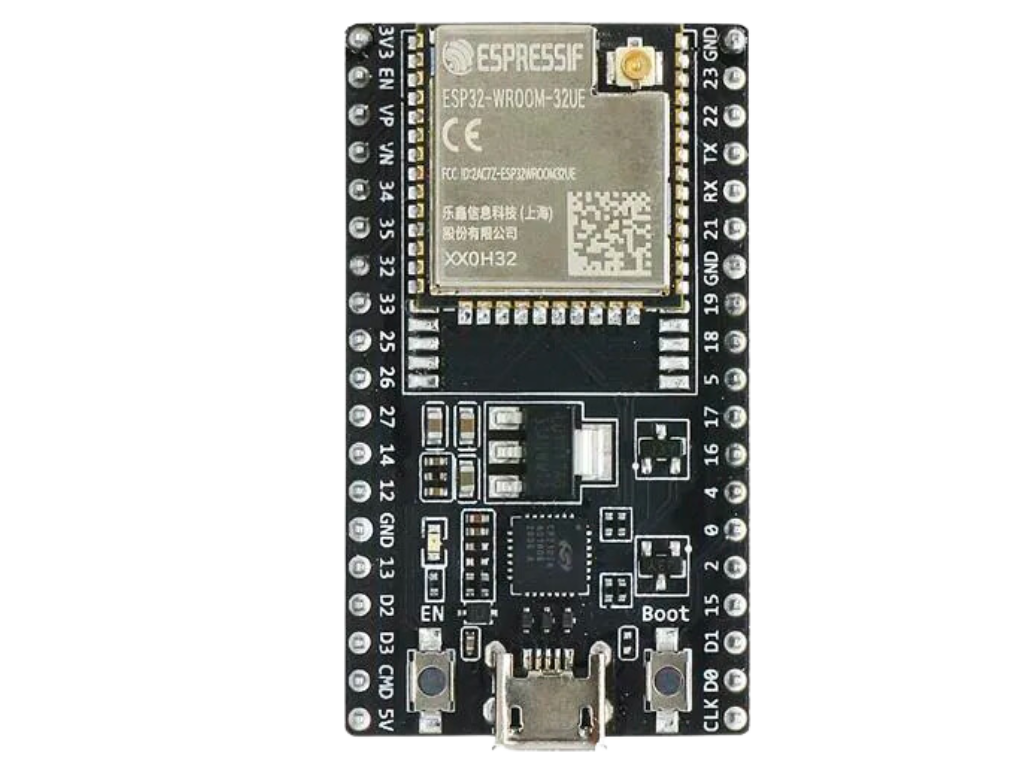
\includegraphics[width=\linewidth, angle=360]{pics/esp32.png}
    \end{minipage}\hfill
    \caption{NodeMCU ESP32 and its specifications}\label{tab:nodemcu}
\end{table}



\newpage


\subsubsection{Motor Controller}

\vspace{-0.6em}

Since the robot will be navigating in a hospital environment, electric motors will be used for this
application as they reduce noise level and CO$_2$ emissions. This also fulfills the ISO 23482-2:2019 which provides guidance
on new safety terms and requirements to enable close human-robot interaction. The motors will be controlled by an L298N motor driver. The
XH-M249 / XY-3606 steps down the voltage from battery 24V to 5V for the microcontrollers and other components.

\vspace{1em}


\begin{table}[h]
    \begin{minipage}{0.6\textwidth}
        \centering
        \renewcommand{\arraystretch}{2.0}
        \setlength{\tabcolsep}{4.4pt}
        \footnotesize
        \begin{tabular}{|p{4.5cm}|p{4.5cm}|}
          \hline
          \rowcolor[gray]{0.8} 
          \textbf{Parameter} & \textbf{Value} \\
          \hline
          Driver Chip &  Double H Bridge L298N \\
          \hline
          Motor Supply Voltage (max) & 46V \\
          \hline
          Motor Supply Current (max) & 2A \\
          \hline
          Logic Voltage & 5V \\
          \hline
          Driver Voltage & 5V -- 35V \\
          \hline
          Logic Current & 0 -- 36mA \\
          \hline
          Driver Current & 2A \\
          \hline
          Maximum Power & 25W \\
          \hline
        \end{tabular}
    \end{minipage}
    \begin{minipage}{0.36\textwidth}
        \centering
        \includegraphics[width=\linewidth, angle=360]{pics/l298n.png}
    \end{minipage}\hfill
    \caption{L298N Motor Driver and its specifications}\label{tab:l298n}
\end{table}

\vspace{-0.4em}


\begin{table}[h]
    \begin{minipage}{0.6\textwidth}
        \centering
        \renewcommand{\arraystretch}{2.0}
        \setlength{\tabcolsep}{4.4pt}
        \footnotesize
        \begin{tabular}{|p{4.0cm}|p{5.0cm}|}
          \hline
          \rowcolor[gray]{0.8} 
          \textbf{Parameter} & \textbf{Value} \\
          \hline
          Driver Chip &  XH-M249 / XY-3606 \\
          \hline
          Input Voltage & DC 9V -- 36V \\
          \hline
          Output Voltage & 5.2V / 5A / 25W \\
          \hline
          Output Voltage & $V_{out} = 5V$ DC ($V_{in} \geq V_{out} + 1.5V$) \\
          \hline
          Output capability & Input: 9 $\sim$ 24V  \newline Output: 5.2V / 6A / 30W \\
          
           & Input: 24 $\sim$ 32V \newline  Output: 5.2V / 5A / 25W \\
          
           & Input: 32 $\sim$ 36V \newline Output: 5.2V / 3.5A / 18W \\
          \hline
          Size & 63 * 27 * 10cm (L * W * H) \\
          \hline
        \end{tabular}
    \end{minipage}
    \begin{minipage}{0.36\textwidth}
        \centering
        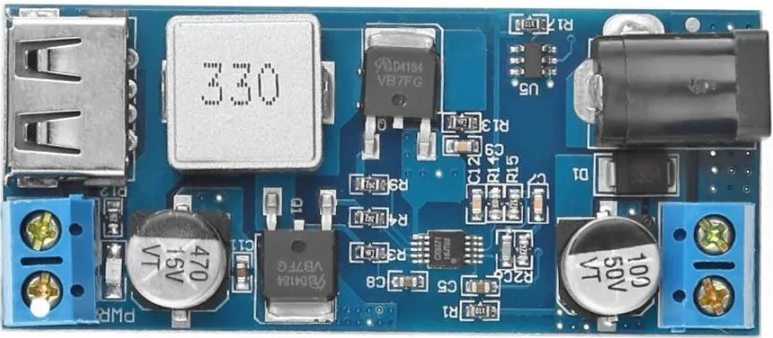
\includegraphics[width=\linewidth, angle=90]{pics/xr.png}
    \end{minipage}\hfill
    \caption{DC Step Down XH-M249 / XY-3606 and its specifications}\label{tab:l298n}
\end{table}




\newpage
\subsection{Software Implementation}

\subsubsection{Ecosystem}
This project uses a sophisticated software ecosystem to achieve autonomous navigation and medicine dispensing. The Robot Operating System 2 (ROS2) is the middleware, enabling seamless communication and integration between various software components. 

\vspace{0.4in}

\begin{figure}[H]
    \centering
    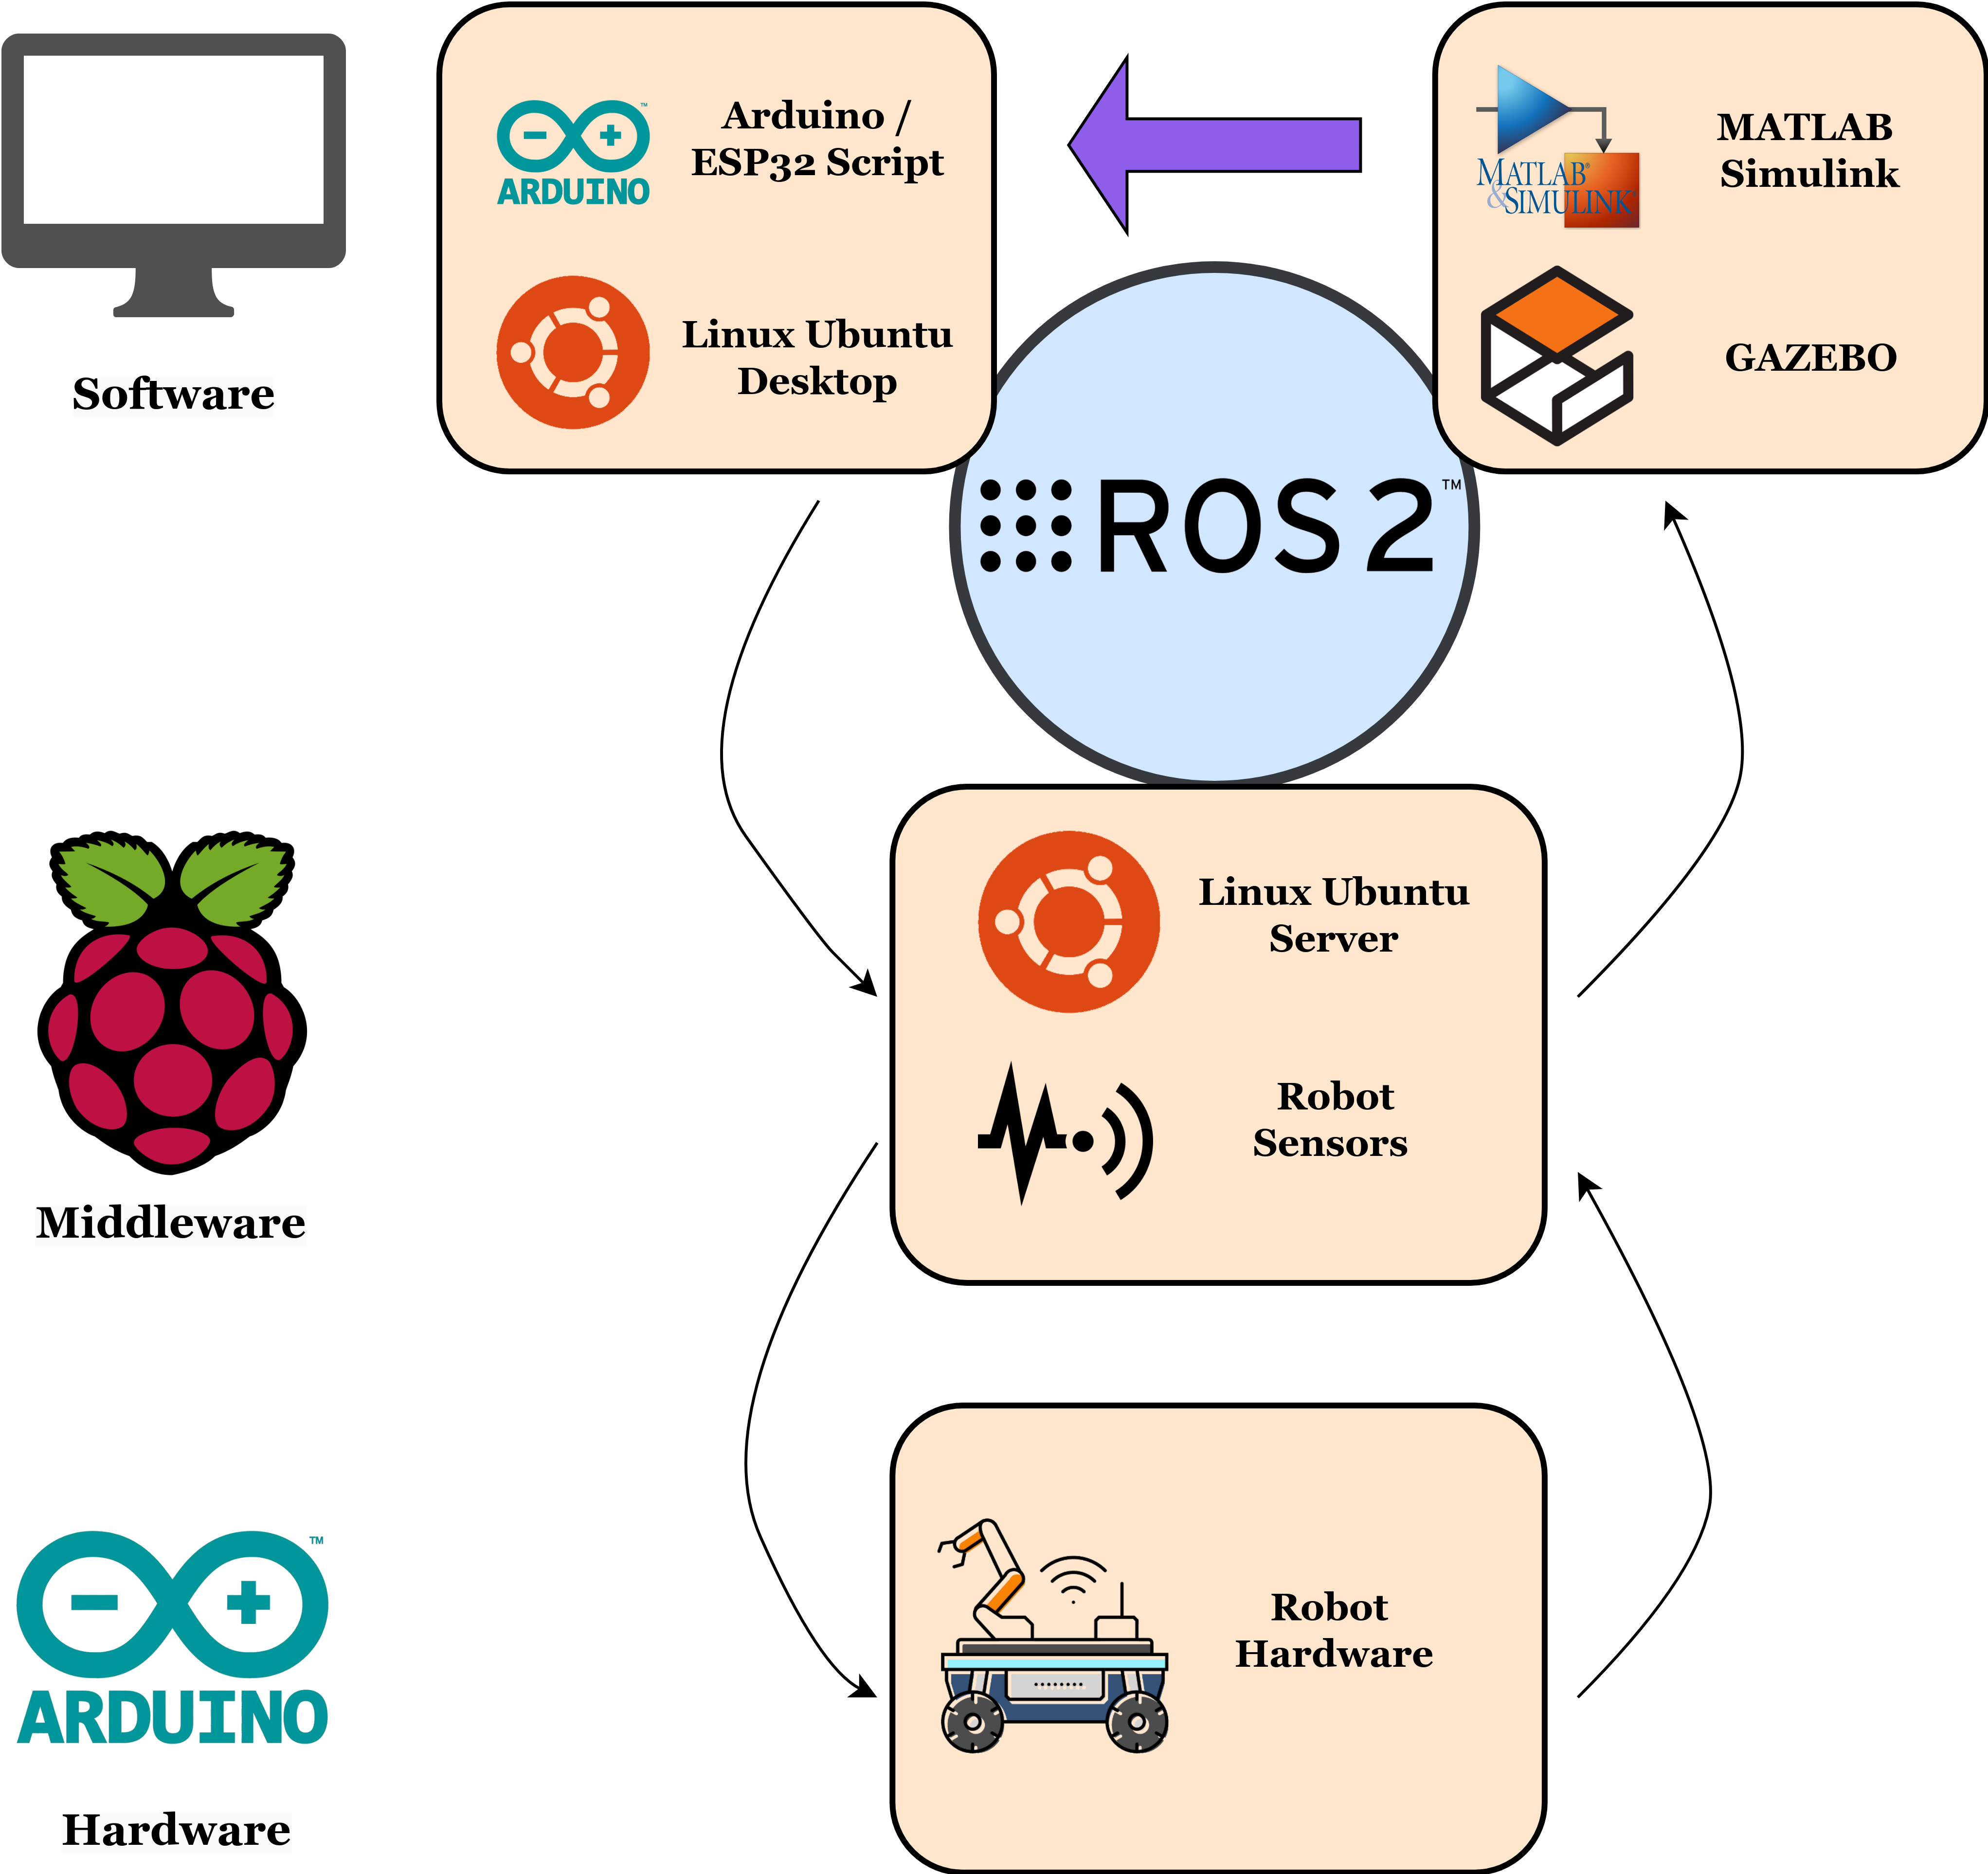
\includegraphics[width=6.2in]{pics/illustration.png}
    \caption{ROS2 Ecosystem}\label{ros2}
\end{figure} 

\vspace{0.4in}


\noindent A headless Raspberry Pi 4, running an Ubuntu server and ROS2 Humble Hawksbill, acts as the central processing unit. This configuration optimizes computational resources by eliminating the overhead of a graphical user interface. The Raspberry Pi communicates with an ESP32 microcontroller, which handles low-level control functions like motor control and sensor data acquisition.
ROS2's node architecture facilitates the integration of sensor data from the LiDAR, IMU sensor, encoder wheels, ultrasonic and Time of Flight sensors. This data is then processed and visualized using a combination of Gazebo and RViz2. These tools provide a view of the robot's environment and its interactions. MATLAB's Simscape and Simulink tools could also be integrated with ROS2 to offer an alternative visualization method and enable potential future utilization of MATLAB's extensive capabilities.
A vital aspect of this project is the development of a "digital twin." This digital twin will mirror the actions and movements of the physical robot in a simulated environment. This approach allows for real-time remote feedback and facilitates virtual simulations, enabling the testing and refinement of navigation algorithms without relying solely on physical trials. This not only accelerates the development process but also conserves resources and energy.





\subsubsection{User Interface} 
User interface is an important part of the robot system as the robot has to meet basic safety standards and also, it has
to interact easily with the operator. This interface will comprise of switches for user input mounted on the robot, as well as
a Graphical User Interface (GUI) on the workstation computer for remote monitoring and control. Subsequently, the ISO 15066:2016 standard defines safe ways in which 
humans can interact with robots. It mandates the necessity of including emergency stop mechanisms. As such, the signal shall be an emergency switch infront of the robot
which is very accessible. When pressed, the robot will halt and stop all movement operations. To interact with the robot's navigation 
and mapping system, most of the
operations can be achieved through a terminal-driven interface, but a graphical user interface (GUI) will be more
intuitive and user-friendly especially for non-technical users. There are several tools and external softwares
e.g Foxglove, that can be adapted to develop the user interface. However, building a custom GUI offers more control
and flexibility in terms of design and functionality. Qt is a cross-platform application framework used for developing
GUIs. Qt supports C++ and integrates well with ROS2, hence it is chosen for this project. 

\subsubsection{System Architecture}
The system architecture of the autonomous medicine dispensing robot, as shown in the Figure~\ref{system} below, comprises
a network of interconnected hardware and software components. The power system, driven by a 24V 22Ah LiPo battery, supplies
energy to the robot. A DC-DC buck converter (XH-M249) steps down this voltage to 12V and 5V to power various components, including the processing
units and sensors. The primary processing unit is a Raspberry Pi 4B 8GB. It communicates with an Arduino UNO 
via UART, delegating low-level control functions such as motor control and encoder data acquisition. An ESP32
is also integrated into the system, which connects wirelessly
with the Raspberry Pi.
The robot's sensing system includes a 2D RP-LIDAR A1 M8 for 360-degree environmental scanning, three HCR-S04 ultrasonic sensors
for perimeter obstacle detection, a VL53L0X V2 Time-of-Flight sensor for precise frontal distance measurement, an MPU9250 IMU 
for motion sensing, and an NTC temperature sensor for thermal monitoring. Actuation is achieved through an L298N motor driver,
which controls two motors equipped with encoders for precise movement. Cooling fan ensure the electronics maintain a safe operating temperature.
Communication within the system is facilitated through various protocols, including UART for short-range connections, SSH
for secure remote access to the Raspberry Pi, and Wi-Fi (TCP/IP) for wireless
communication with the GUI workstation. A USB hub could expand the Raspberry Pi's connectivity options, especially when debugging,
but it is unnecessary when the robot operates. The user interface comprises a keypad, extra switches on the robot itself, and
a GUI workstation for more complex user interactions and monitoring. 

\vspace{0.15in}

\begin{figure}[H]
    \centering
    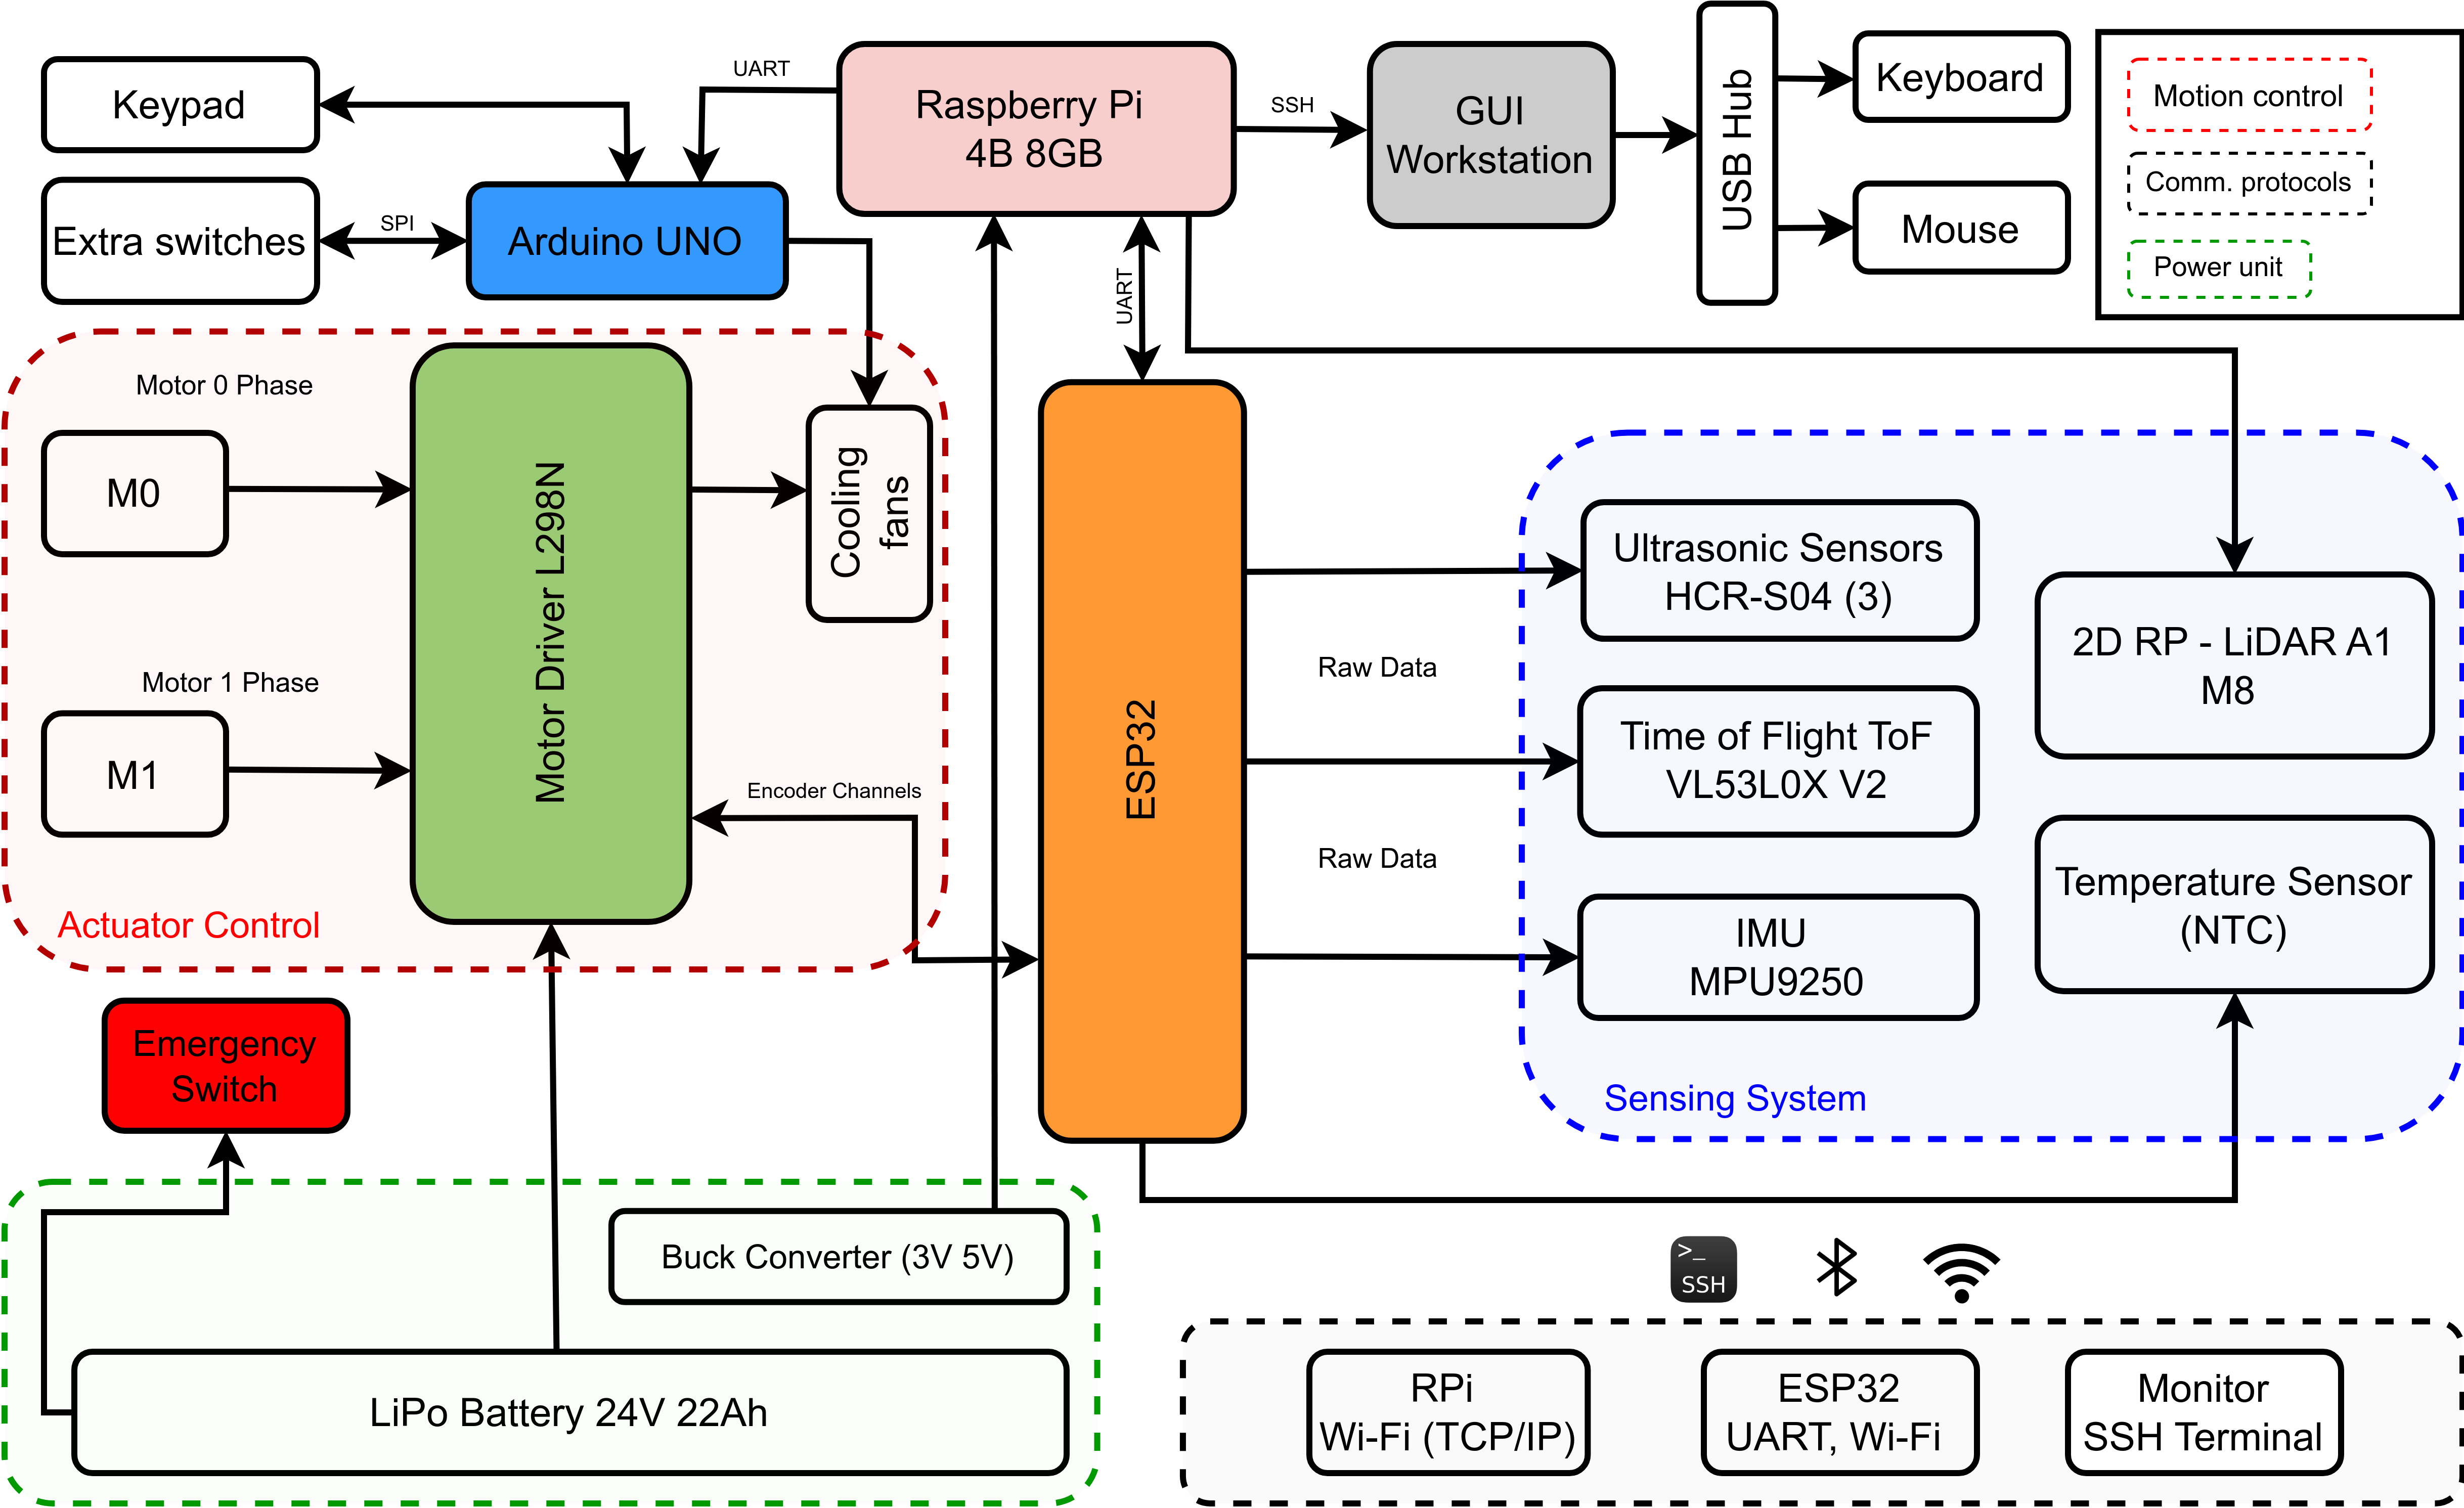
\includegraphics[width=6.1in]{pics/Hardware_Architecture3.png}
    \caption{System Architecture Overview}\label{system}
\end{figure} 


